\documentclass[a4paper]{article}

\usepackage[english]{babel}
\usepackage[utf8]{inputenc}
\usepackage{amsmath}
\usepackage{graphicx}
\usepackage[colorinlistoftodos]{todonotes}

\newcommand{\figref}[1]{Fig.~\ref{fig:#1}}

\title{Physiological Modeling For Closed-loop Validation of Medical Devices}

\author{You}

\begin{document}
\maketitle

\begin{abstract}
Your abstract.
\end{abstract}

\section{Closing the Device-Patient Loop}
Medical devices operate across a range of invasiveness and intervention with the patient in the loop. For diagnostic-only devices, e.g. an X-ray machine, the physician operates the device to obtain patient data, perform diagnosis and deliver proper therapy to the patient (\figref{closed-loop}.(a)). For therapy-only devices, e.g. a drug infusion pump, the physician configures the device infrequently based on prior diagnosis of the patient so the device executes the therapy on the patient (\figref{closed-loop}.(b)). We denote these devices as \textbf{Open-loop Medical Devices} as there is no direct feedback between the patient and the device. For open-loop devices, the device operates under the supervision of professionally-trained physicians. The device's safety is determined by how accurately it provides information to the physicians and its faithful operation as instructed by the physicians.

There is a class of devices with both diagnostic and therapeutic functions, i.e. implantable cardiac devices to treat cardiac arrhythmia, deep brain stimulation devices (\cite{Brain_sti}) to treat Parkinson's disease and artificial pancreas to treat Type 1 diabetes. These devices capture and diagnose the patient's physiological conditions from sensory data, and deliver therapy in response (\figref{closed-loop}.(c)). These devices usually operate (semi-) autonomously with very little human intervention, thus malfunctions or inappropriate therapies from these devices cannot be corrected timely, which can cause serious adverse effects on patients' health. Therefore these devices are usually classified into the highest risk category and undergo the most stringent regulation. We denote them as \textbf{Closed-loop Medical Devices}. 
\begin{figure}[t]
		\centering
		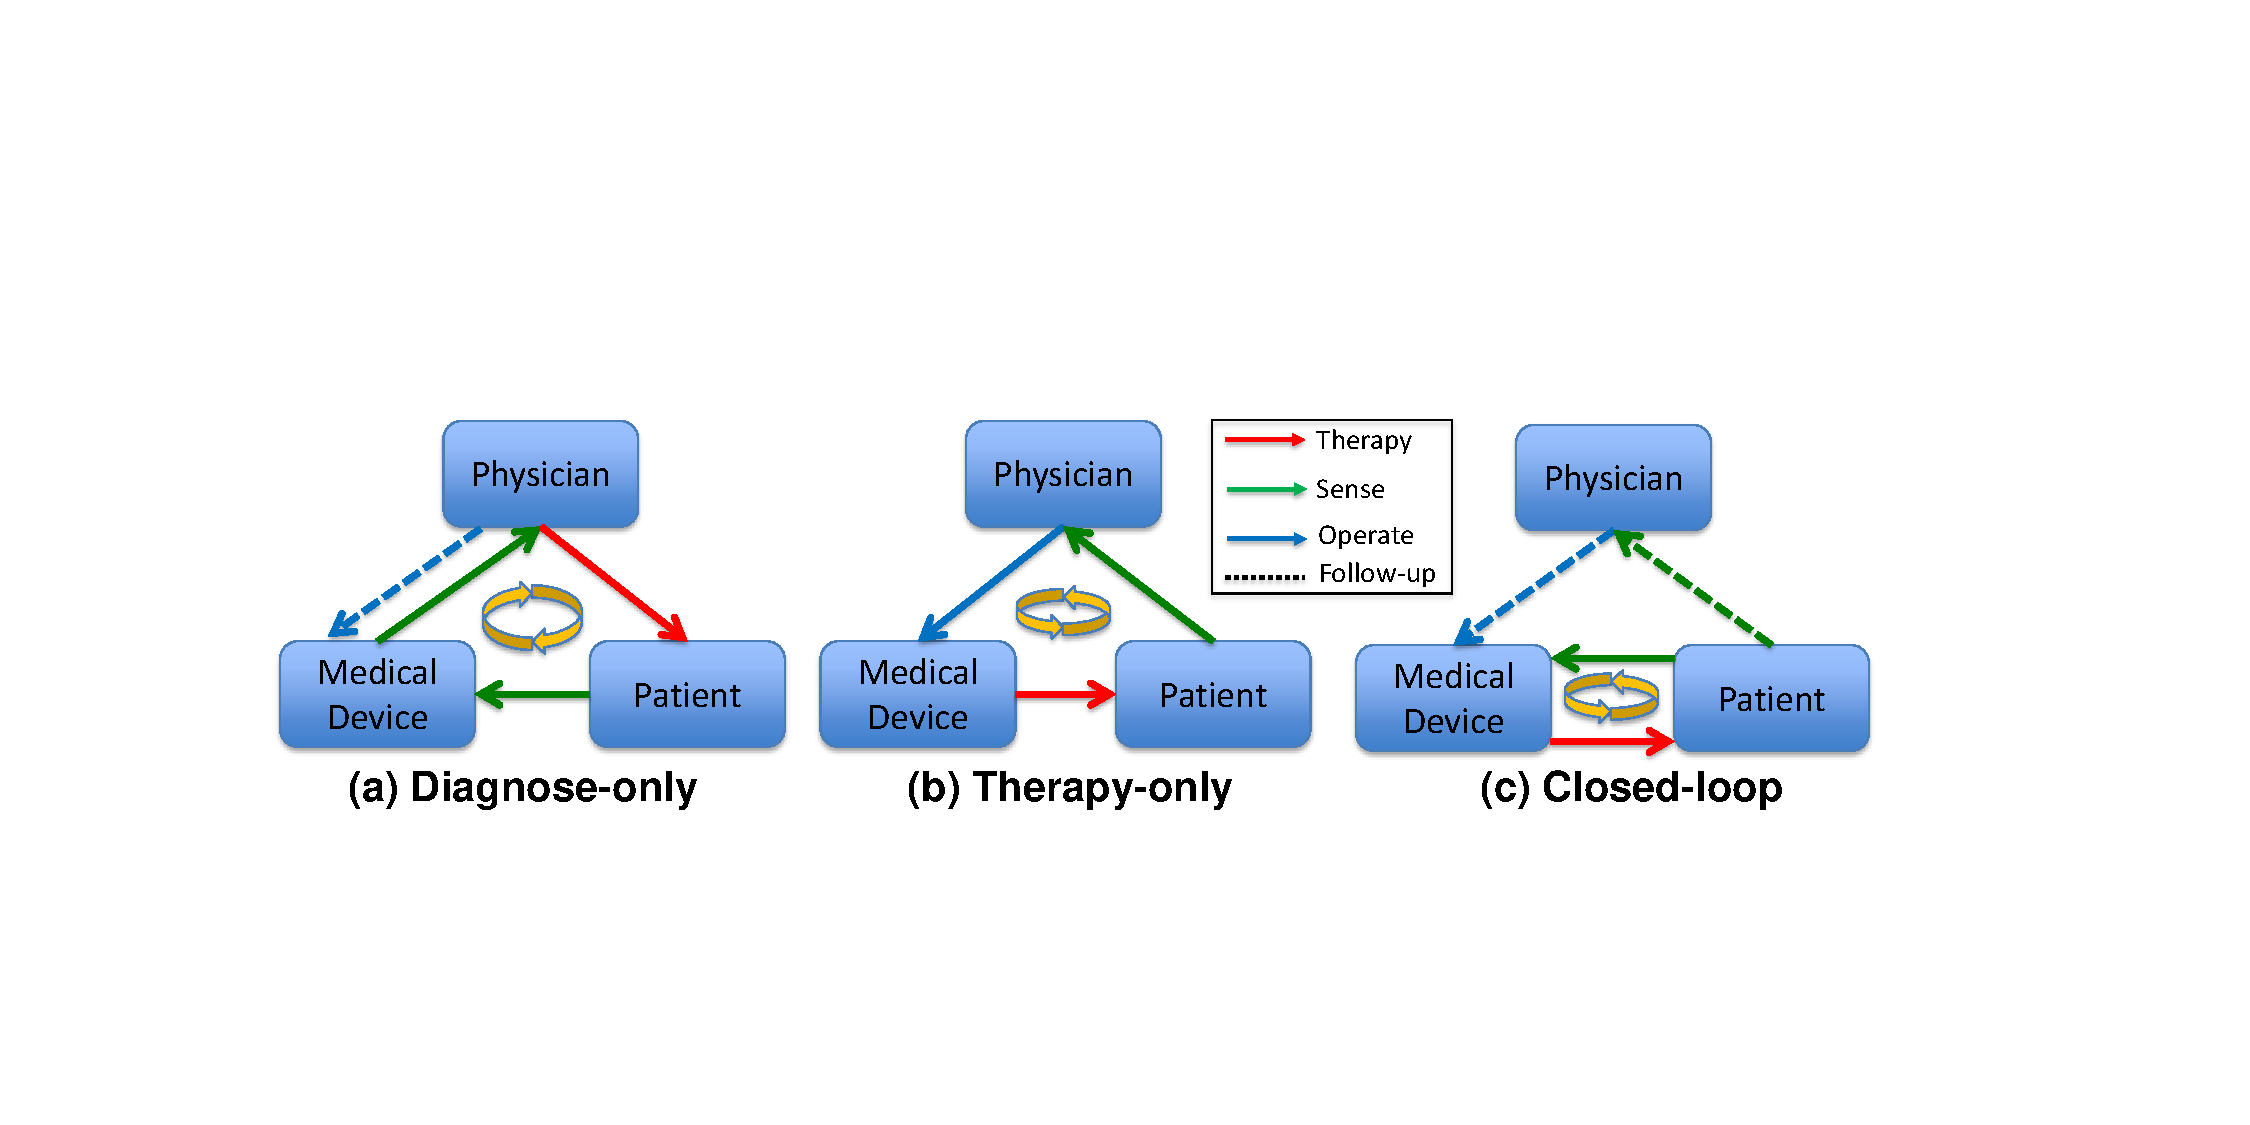
\includegraphics[width=\textwidth]{figs/closed-loop.pdf}
		\caption{\small Diagnostic-only and therapy-only devices do not interact with the patient in direct closed-loop. The physician is responsible for the diagnostic and/or therapeutic decisions. However in closed-loop medical devices, the devices interact with the patient in closed-loop and have to make therapeutic decisions based on their own diagnosis.}
		\label{fig:closed-loop}
\end{figure}
There are multiple challenges to develop safe and effective closed-loop medical devices:

\subsection{Closed-loop Interactions with Complex Physiology}
When using open-loop medical devices, the diagnosis and therapy decisions are made by medical professionals, who have expert knowledge of human physiology. Therefore they are able to identify adverse health conditions and adjust the therapy accordingly. On the other hand, closed-loop medical devices have to make both the diagnosis and therapy decisions on their own. The domain expertise required to make those decisions has to be programmed into the device. It is impossible to encode all the knowledge of human physiology into the device. Therefore, for unanticipated physiological conditions when the appropriate response has not been programmed into the device, the device may deliver inappropriate therapy which can cause adverse effect on patient's health. 

Technological development of materials, sensors, embedded computing, energy storage, communications and packaging usher new closed-loop therapies (e.g. deep brain stimulation). While the spectrum of closed-loop interactions between the device and the human physiology may not be fully understood, the challenge is to ensure the device never drives the patient into an adverse state. Furthermore, even with well-understood behaviors, with the incremental addition of new therapies in legacy devices (e.g. cardiac rhythm therapy), may result in inadvertent and conflicted behavior ending up with inappropriate and unsafe operation. 

\subsection{Limited Diagnostic and Therapeutic Functions}
One fundamental rationale behind closed-loop medical devices is to enable the patients to live their normal lives without the dependance of cumbersome medical devices and with minimal physician supervision. In fact, a large number of closed-loop medical devices are autonomous implantable devices. As a result, the sensing and therapy capabilities of the devices are limited, in order to minimize power consumption, heat dissipation and invasiveness. Limited sensing capabilities may cause misdiagnosis as the device may be unable to distinguish the source between two sensed signals from different conditions that now seem similar and result inappropriate therapy. Due to limited therapeutic capabilities, there exists sub-optimal physiological conditions that are untreatable. The device may even trigger the conditions into less optimal conditions. In later chapters we will describe examples in which an untreatable condition is deteriorated into an adverse condition due to device interactions.

\subsection{Software-related Medical Device Recalls}
Due to the complexity of the diagnostic and therapeutic functions of the closed-loop devices, these functions are mostly controlled by their software components. 
Software embedded in a medical device, unlike electrical and mechanical components, does not fail due to corrosion, fatigue or have statistical failures of subcomponents. Software failures are uniquely sourced in the design and development of the system. %Unlike other industries such as consumer electronics where product life cycles are measured in months, software engineering for medical devices often spans a decade and must prioritize safety and efficacy over time to market. 
%\begin{figure}[t]
		%\centering
		%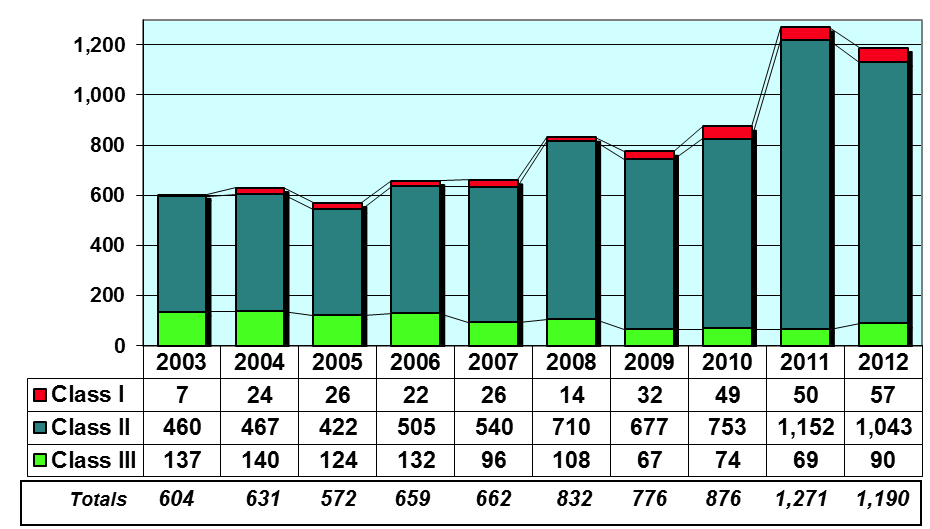
\includegraphics[width=0.8\textwidth]{figs/recalls.jpg}
		%\caption{\small Medical device recalls have risen over the past decade}
		%\label{fig:recalls}
%\end{figure}
\begin{figure}[t]
		\centering
		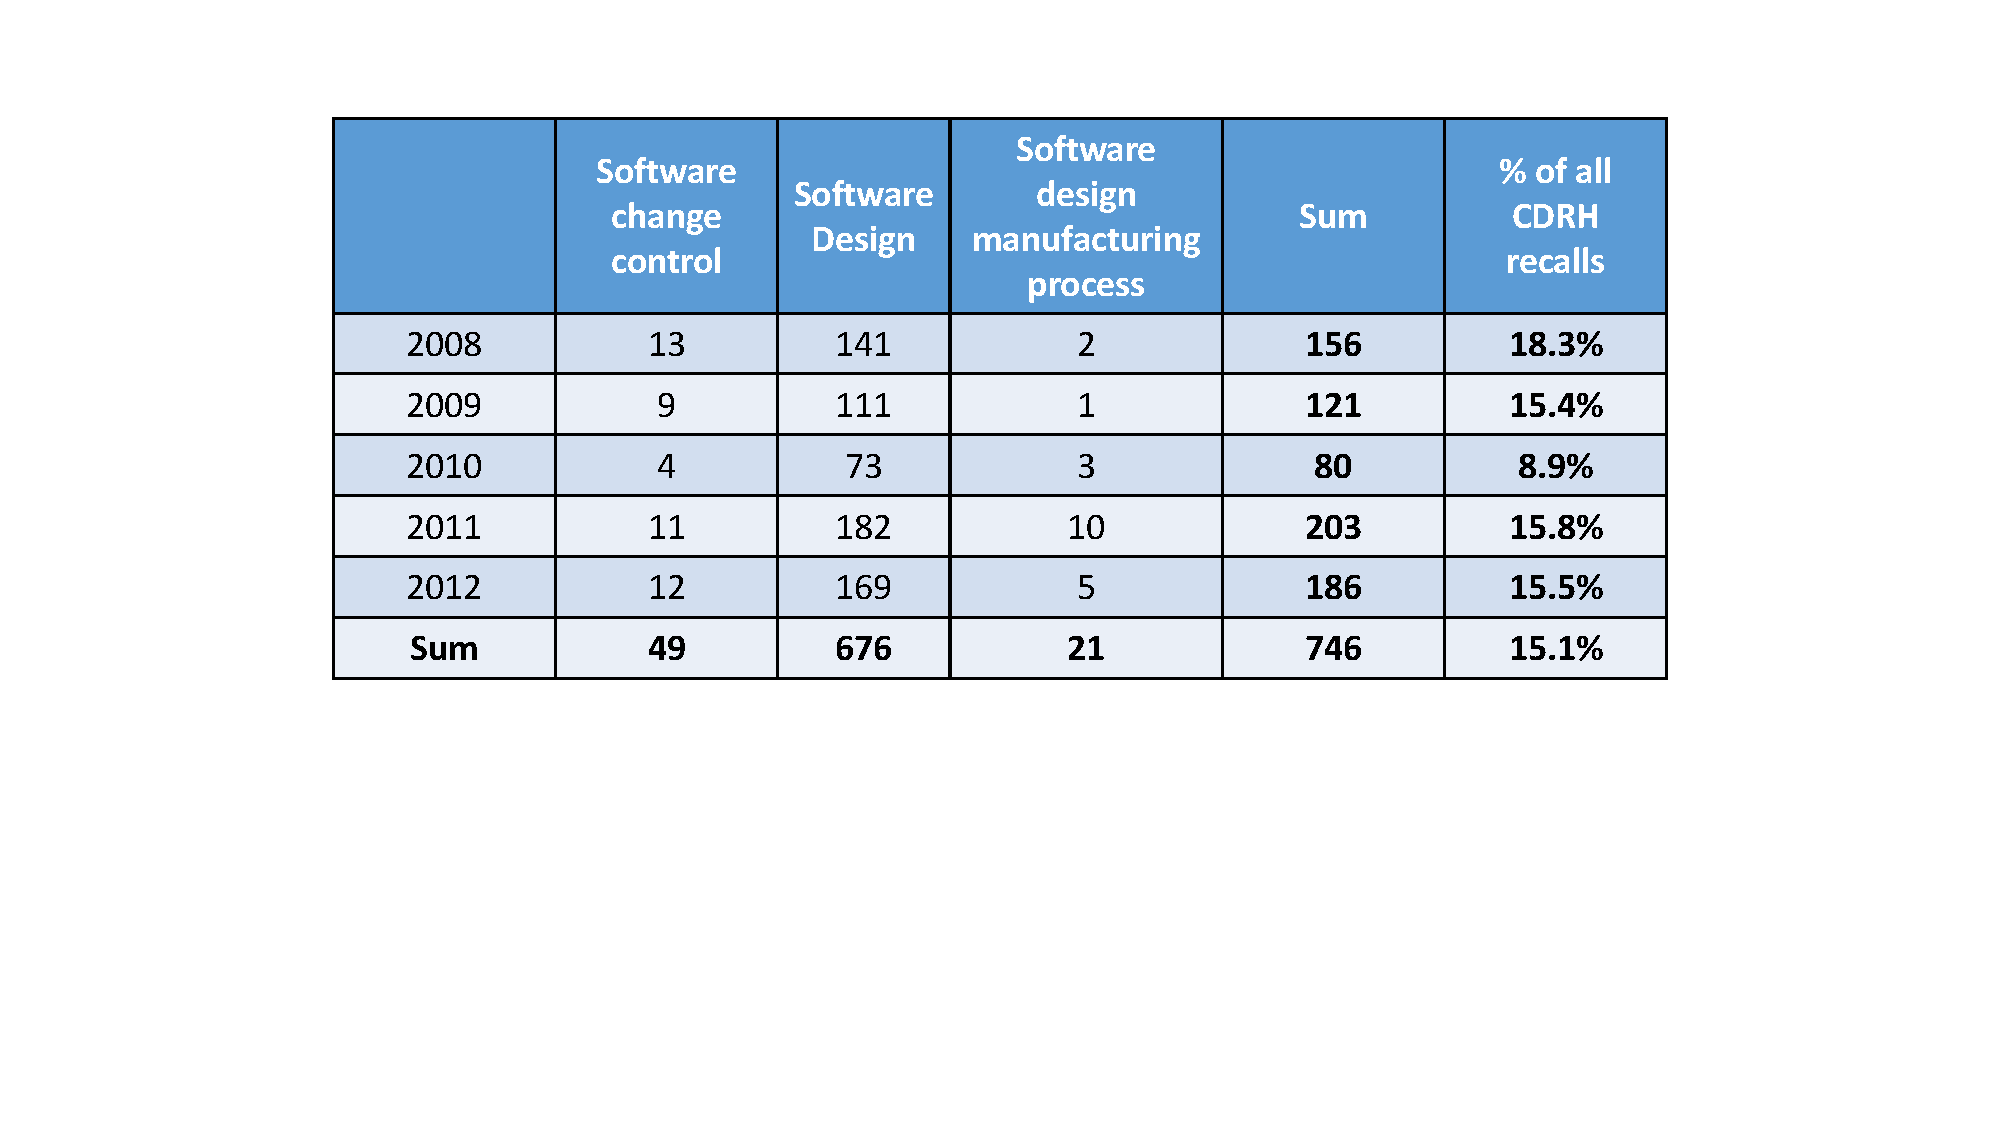
\includegraphics[width=0.8\textwidth]{figs/recalls.pdf}
		\caption{\small Medical device recalls due to software issues have risen from 10\% in the 1990s to \~15\% in the past decade (\cite{recall_rep})}
		\label{fig:soft_recalls}
\end{figure}
%  Over the course of the past four decades, cardiac rhythm management devices such as pacemakers and implantable cardioverter defibrillators (ICD) have grown in complexity and now have more than 80,000 to 100,000 lines of code (\cite{pauljones}). 
According to the US Food and Drug Administration, in 1996, 10\% of all medical device recalls were caused by software-related issues (\cite{medstats}). This percentage rose to an average of 15\% of recalls from 2008 to 2012 (\figref{soft_recalls}). Malfunctions of closed-loop medical devices usually have severe consequences, which will be categorized as \emph{Class I}, meaning there is a ``reasonable probability that use of these products will cause serious adverse health consequences or death.'' (\cite{medstats2,pacemakerrecalls,killedbycode}). 
\section{Regulation Efforts and Challenges with Medical Devices}
The medical device industry is regulated to ensure the safety of the patients and the public. In the United States, the FDA is the primary regulatory authority responsible for assuring the safety, efficacy and security of patients using medical devices. Based on the rationale that 1) manufacturers know their devices better than the regulator, and 2) the variety of medical devices requires a variety of approaches, it is the device manufacturers' responsibility to demonstrate the safety and efficacy of the medical devices. Manufacturers are required to complete a pre-market submission before the devices can be released to the market. The level of requirements for the submission is determined by the safety classification of the devices. 
\section{Model-based design to improve medical device safety}
With the deluge of software-based closed-loop medical devices in the coming years, relying on clinical trials as the only closed-loop evaluation method to identify risks is not scalable. Model-based design and virtual integration have been proposed and applied in other industries like automotive and avionics (\cite{autosar, avsi}), and can potentially help during the development process and provide extra confidence to the device before conducting clinical trials. However, unlike man-made systems like automobiles and aircrafts, physiological systems are less understood with larger variations. The lack of faithful models of physiological environment of the closed-loop medical devices is one of the reason that model-based design is not well-adopted in the medical device industry. 
\begin{figure}[t]
		\centering
		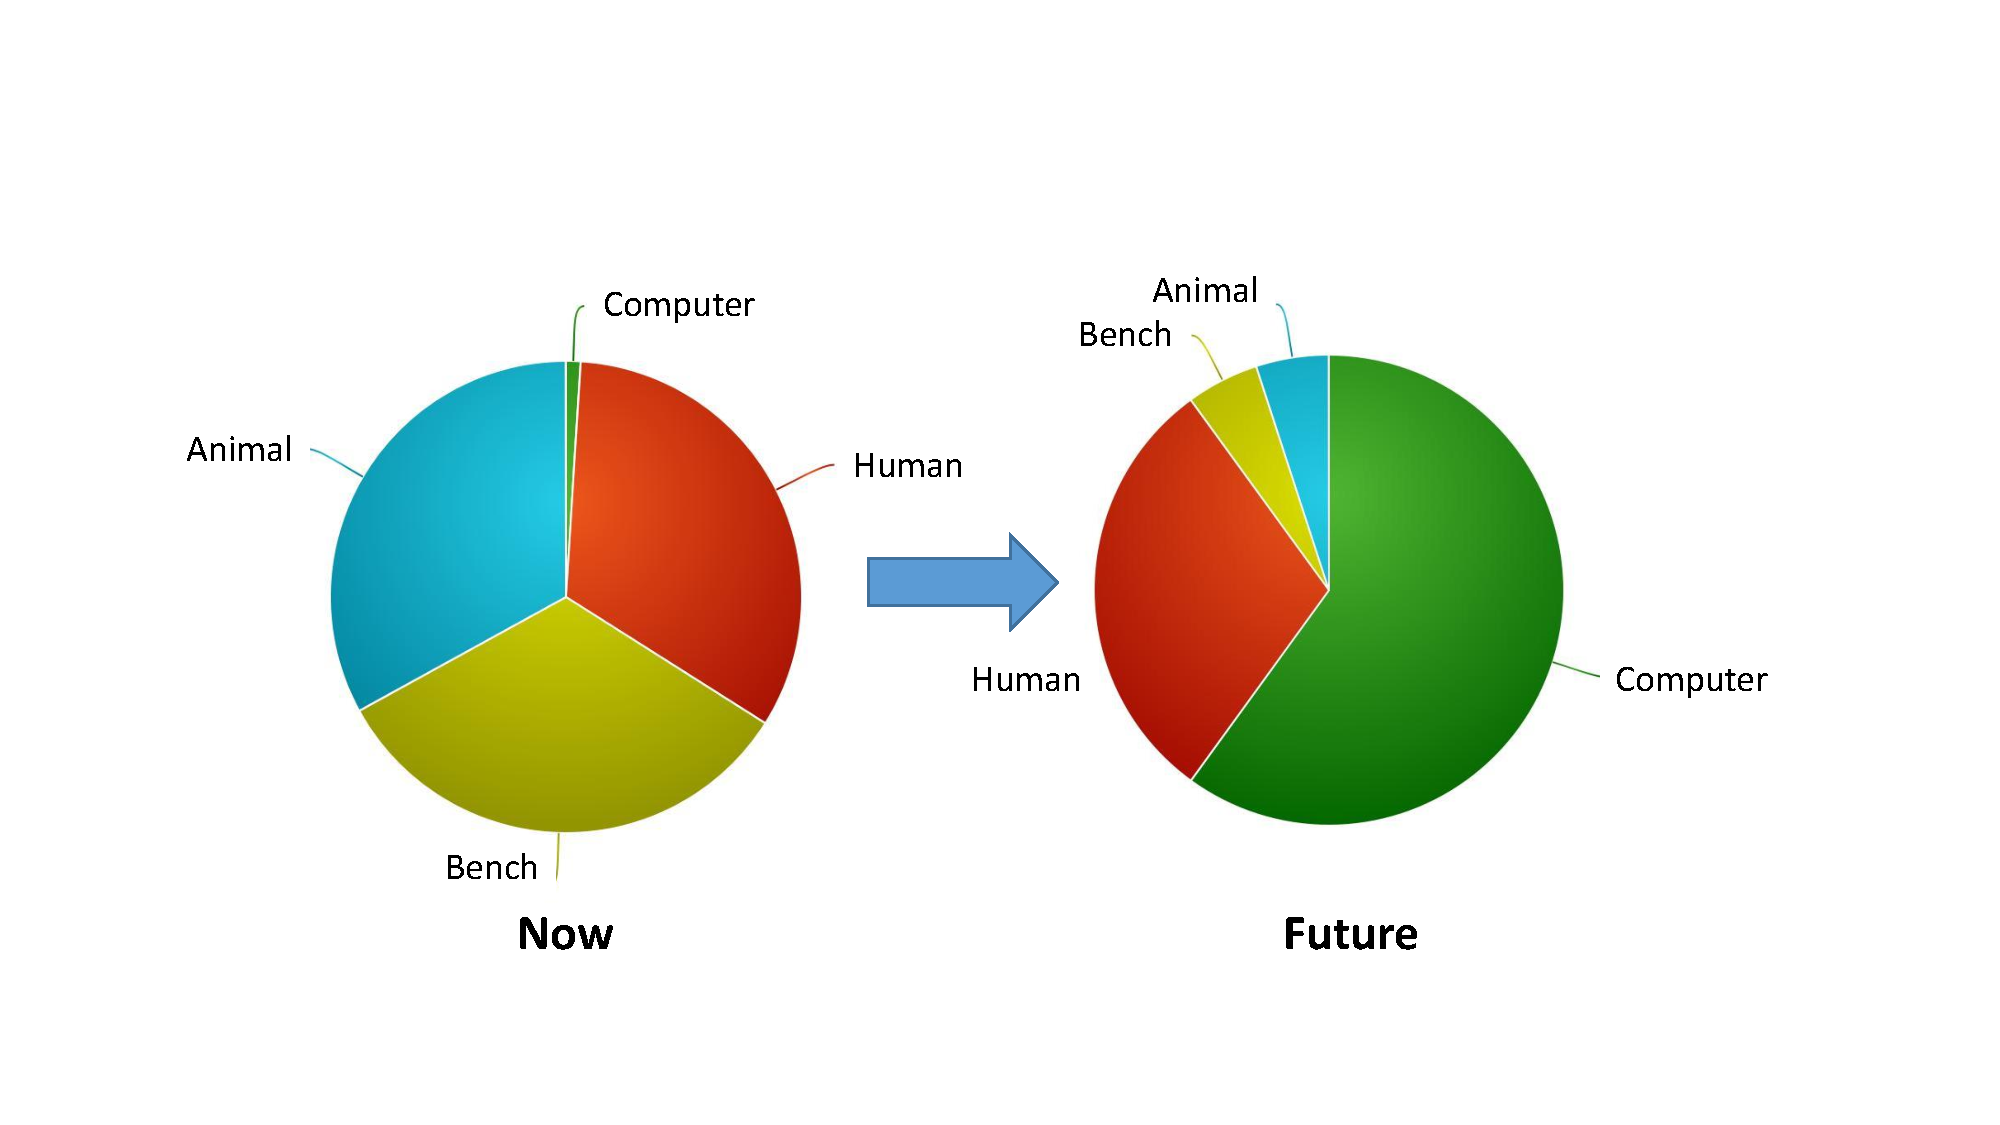
\includegraphics[width=\textwidth]{figs/MDIC.pdf}
		\caption{\small Percentage of computer simulation is expected to increase as safety and effectiveness evidence of medical devices}
		\label{fig:MDIC}
\end{figure}

As computational models of human physiology are developed, they can be used to interact with closed-loop medical devices or their models. The FDA is starting to recognize in silico modeling and simulation as regulatory-grade evidence for device safety and efficacy. For example, \cite{pancreas_paul} developed glucose-insulin models that can be used to evaluate control algorithms for artificial pancreas devices which can sense blood glucose and deliver insulin. Simulation results with the models have been recognized by FDA to replace animal trials, in part, which significantly reduced cost (\cite{pancreas}). With the increasing interest and recognition from the regulators, computer simulations are expected to play bigger role as safety and effectiveness evidence in the development of future closed-loop medical devices (\figref{MDIC}).

\section{Computational Models for Physiological Behaviors}
Closed-loop validation of medical device
\begin{itemize}
	\item As example ,show list of different computational models of the heart (electrical, mechanical, anatomical)
	\item What are their applications? (understand mechanisms, predictions)
	\item Models of organs have really bad prediction performance due to the abstraction of other physiological mechanisms
\end{itemize}

\section{Physiological Models for Closed-loop Evaluation of Closed-loop Medical Devices}
Model simulation results are accepted by FDA as safety evidence (Artificial pancreas)
\begin{itemize}
	\item Key characteristics for interaction with closed-loop medical devices (interface, distinguish conditions, interpretation of execution traces, identifiability)
	\item Why do aforementioned models not suitable for evaluating devices? (unnecessarily complex)
\end{itemize}

\section{Model-based Closed-loop Evaluation of Closed-loop Medical Devices}
Enable closed-loop validation earlier in the development process.
\begin{itemize}
	\item Two applications: Closed-loop Model checking and MBCT
	\item How do they fit into regulation framework

\end{itemize}

\subsection{Closed-loop Model Checking}
Can be used to identify known and unknown mechanisms that can induce hazards.
\begin{itemize}
	\item  Model considerations
	\item Device interface
	\item Coverage vs. Expressiveness
	\item Model refinement
\end{itemize}

\subsection{Model-based Clinical Trials}
Cover target population

\begin{itemize}
	\item Modeling considerations
	\item What is clinical trials and what can they achieve?
	\item What clinical trials cannot achieve? (\textbf{reproducibility}, large population, direct measurement)
	\item How can MBCT help?
\end{itemize}
\section{Outlooks}

\begin{itemize}
	\item Computer simulations are playing more important role as safety and effectiveness evidence for medical devices (\figref{MDIC})
	\item More physiological models designed for device interaction
	\item 
\end{itemize}

\bibliographystyle{plain}
\bibliography{bibliography}
\end{document}